\documentclass[10pt]{article}
\usepackage{graphicx} % Required for the inclusion of images
\usepackage{natbib} % Required to change bibliography style to APA
\usepackage{amsmath} % Required for some math elements 
\usepackage{booktabs}

\title{Assignment 1 report \\ Part A: Experimenting with performance} % Title

\author{Chen Wang, Xiahe Liu (Group 37)} % Author name

\date{\today} % Date for the report

\begin{document}

\maketitle % Insert the title, author and date


% If you wish to include an abstract, uncomment the lines below
% \begin{abstract}
% Abstract text
% \end{abstract}
\section{Hadoop, Tez, Hive (Optional)}

%----------------------------------------------------------------------------------------
%	SECTION 1
%----------------------------------------------------------------------------------------

\section{Experimental Setup}

\subsection{VMs on Azure}
For this assignment 

\subsection{Software}
Hadoop
Tez
Hive


%----------------------------------------------------------------------------------------
%	SECTION 2
%----------------------------------------------------------------------------------------

\section{Mapreduce vs. Tez}
\subsection{Completion time}

\begin{figure}
\begin{center}
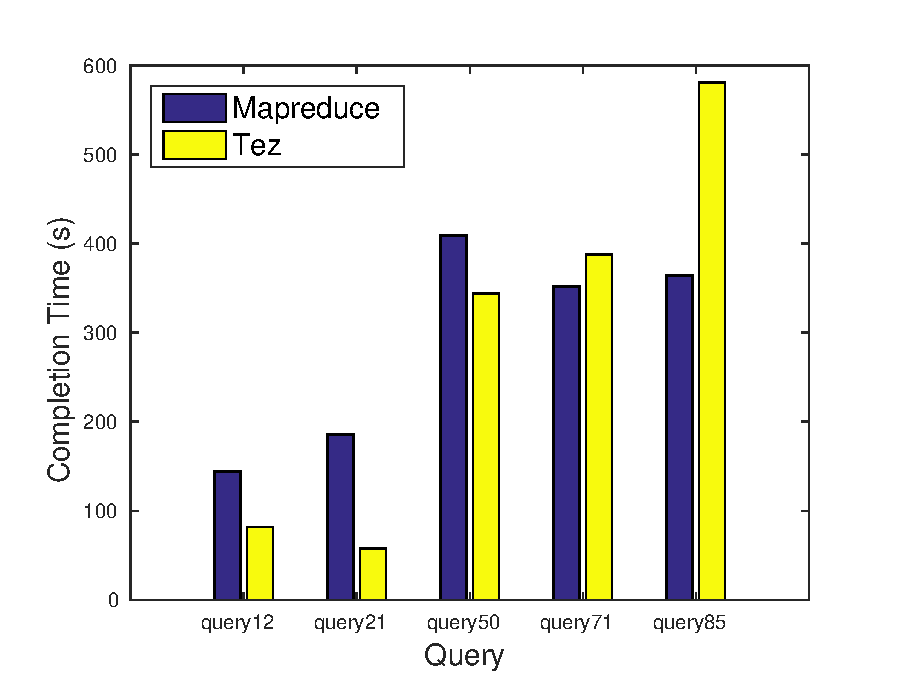
\includegraphics[width=0.75\textwidth]{pic/q1a_time}
\caption{Completion Time of MR and Tez (default parameters).}
\label{fig:q1a_time}
\end{center}
\end{figure}


\subsection{Bandwidth}

\begin{figure}
\begin{center}
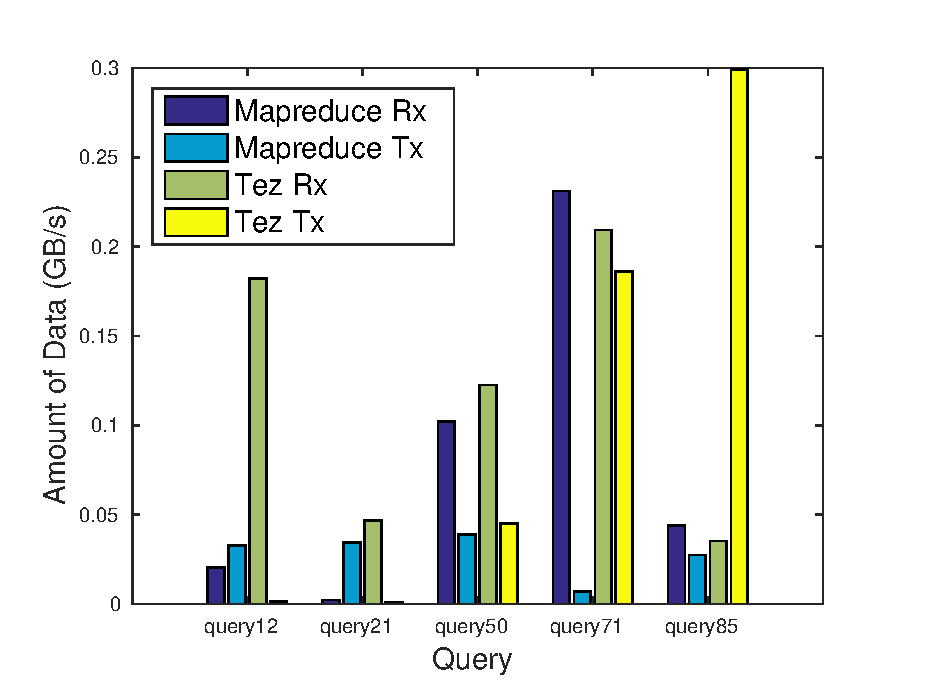
\includegraphics[width=0.75\textwidth]{pic/q1b_net}
\caption{Bandwidth Consumption of MR and Tez (default parameters).}
\label{fig:q1b_net}
\end{center}
\end{figure}

\subsection{Disk}

\begin{figure}
\begin{center}
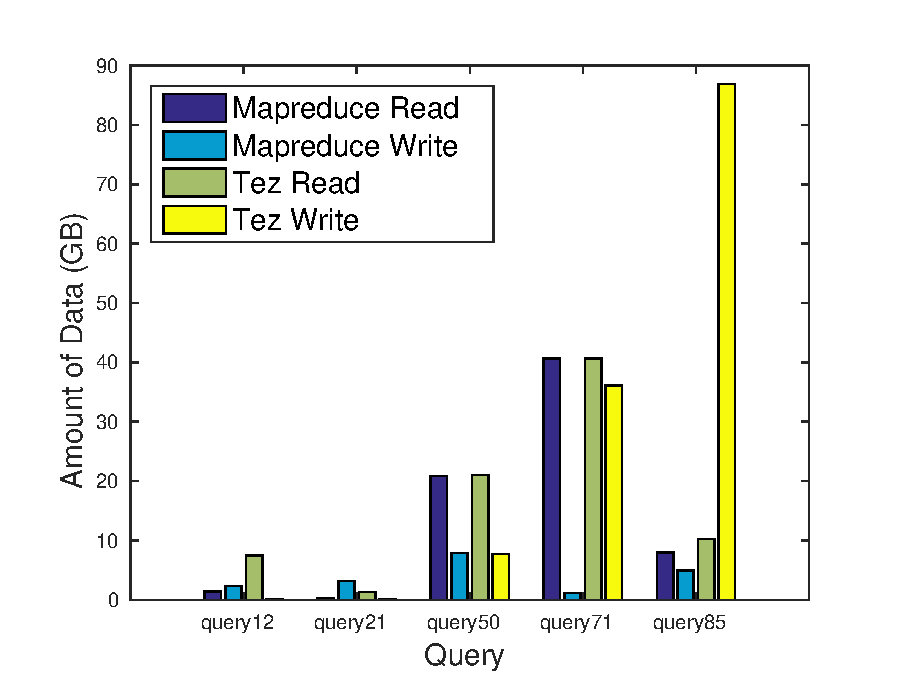
\includegraphics[width=0.75\textwidth]{pic/q1b_disk}
\caption{Disk I/O of MR and Tez (default parameters).}
\label{fig:q1b_disk}
\end{center}
\end{figure}

\subsection{Tasks}

\begin{figure}
\begin{center}
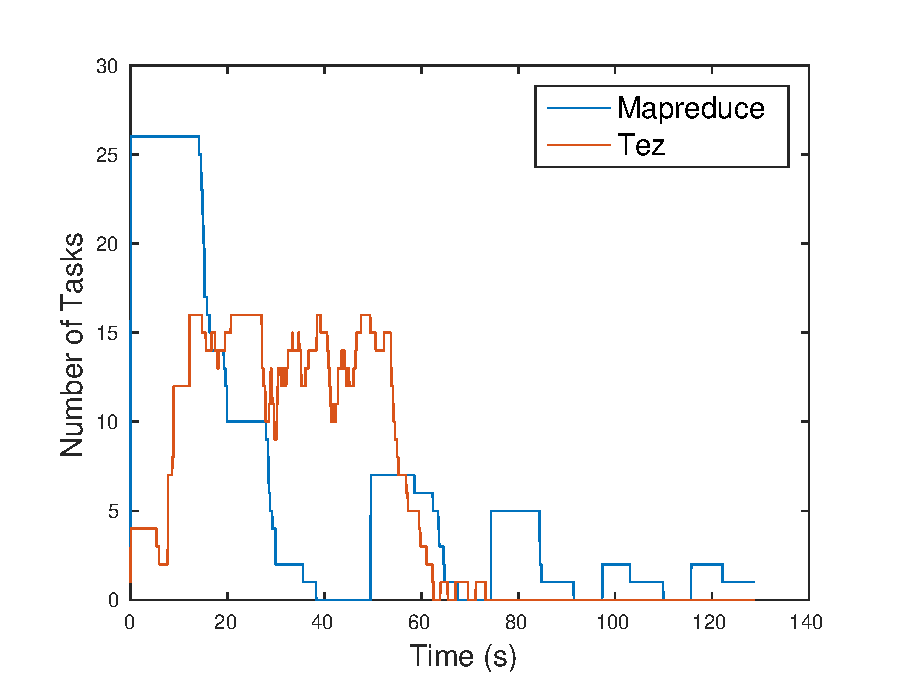
\includegraphics[width=0.75\textwidth]{pic/q1c_task_distribution_12}
\caption{Tasks Distribution over Time (query 12).}
\label{fig:q1c_tasks_12}
\end{center}
\end{figure}

\begin{figure}
\begin{center}
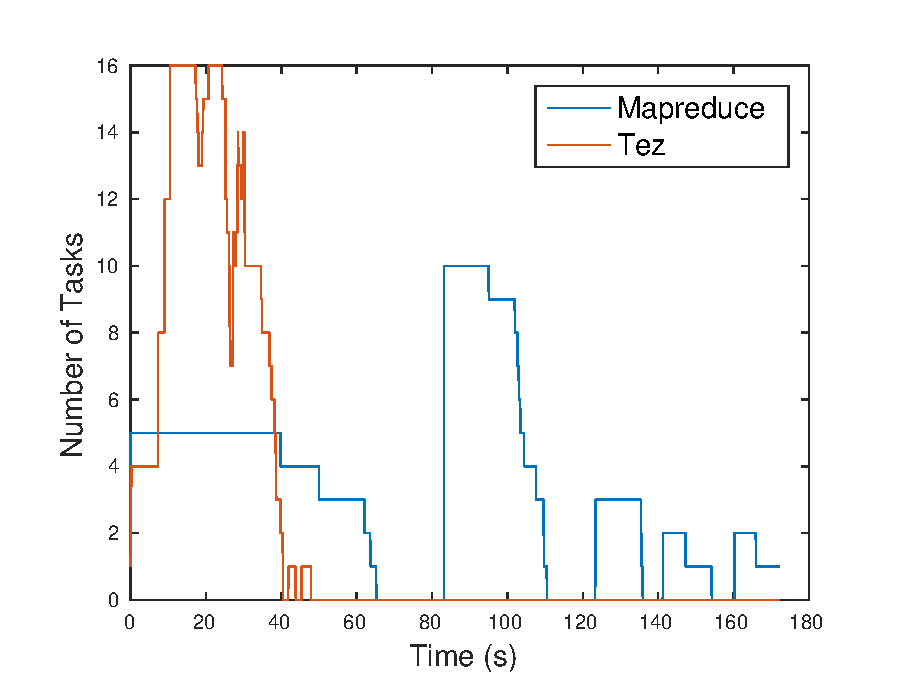
\includegraphics[width=0.75\textwidth]{pic/q1c_task_distribution_21}
\caption{Tasks Distribution over Time (query 21).}
\label{fig:q1c_tasks_21}
\end{center}
\end{figure}

\begin{figure}
\begin{center}
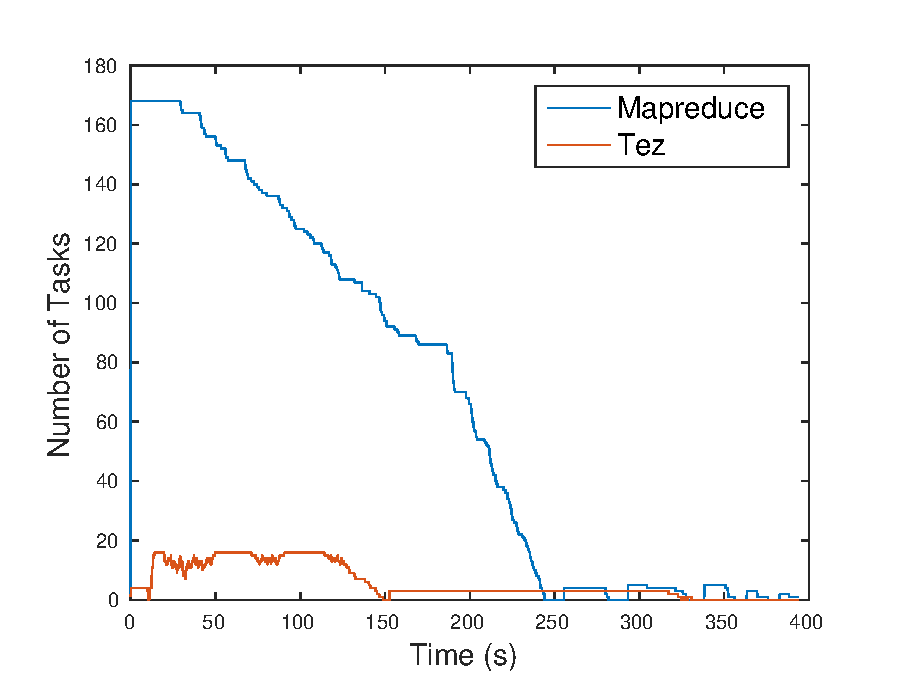
\includegraphics[width=0.75\textwidth]{pic/q1c_task_distribution_50}
\caption{Tasks Distribution over Time (query 50).}
\label{ffig:q1c_tasks_50}
\end{center}
\end{figure}

\begin{figure}
\begin{center}
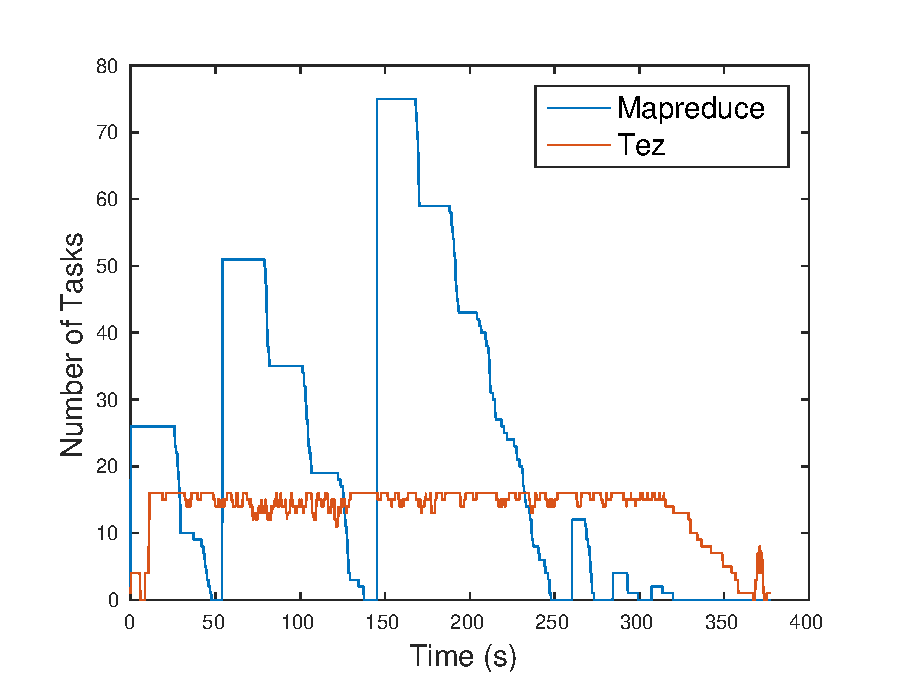
\includegraphics[width=0.75\textwidth]{pic/q1c_task_distribution_71}
\caption{Tasks Distribution over Time (query 71).}
\label{fig:q1c_tasks_71}
\end{center}
\end{figure}

\begin{figure}
\begin{center}
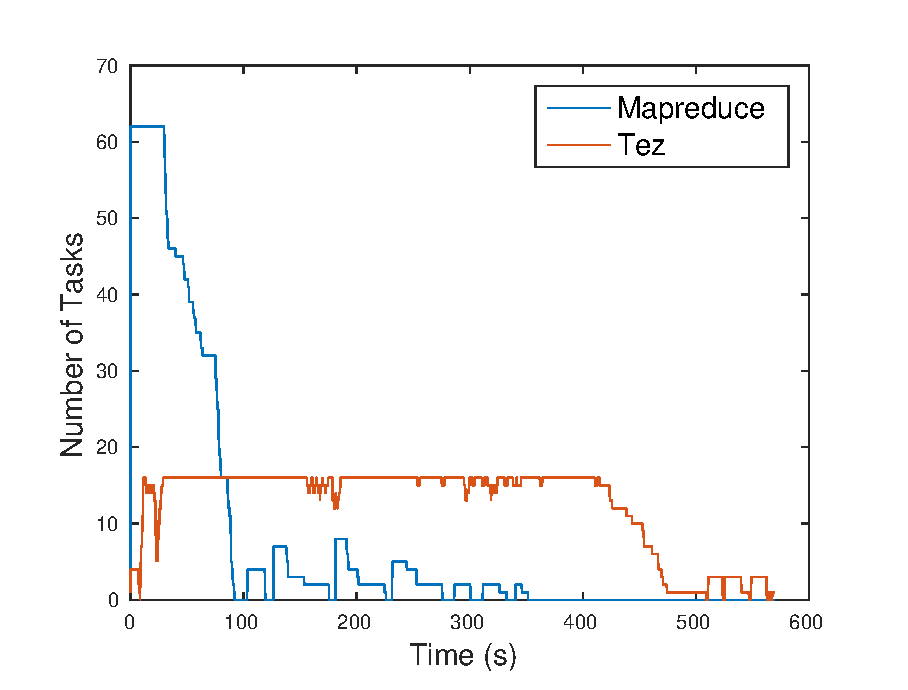
\includegraphics[width=0.75\textwidth]{pic/q1c_task_distribution_85}
\caption{Tasks Distribution over Time (query 85).}
\label{fig:q1c_tasks_85}
\end{center}
\end{figure}


\subsection{Directed Acyclic Graph (DAG)}

\begin{figure}
\begin{center}
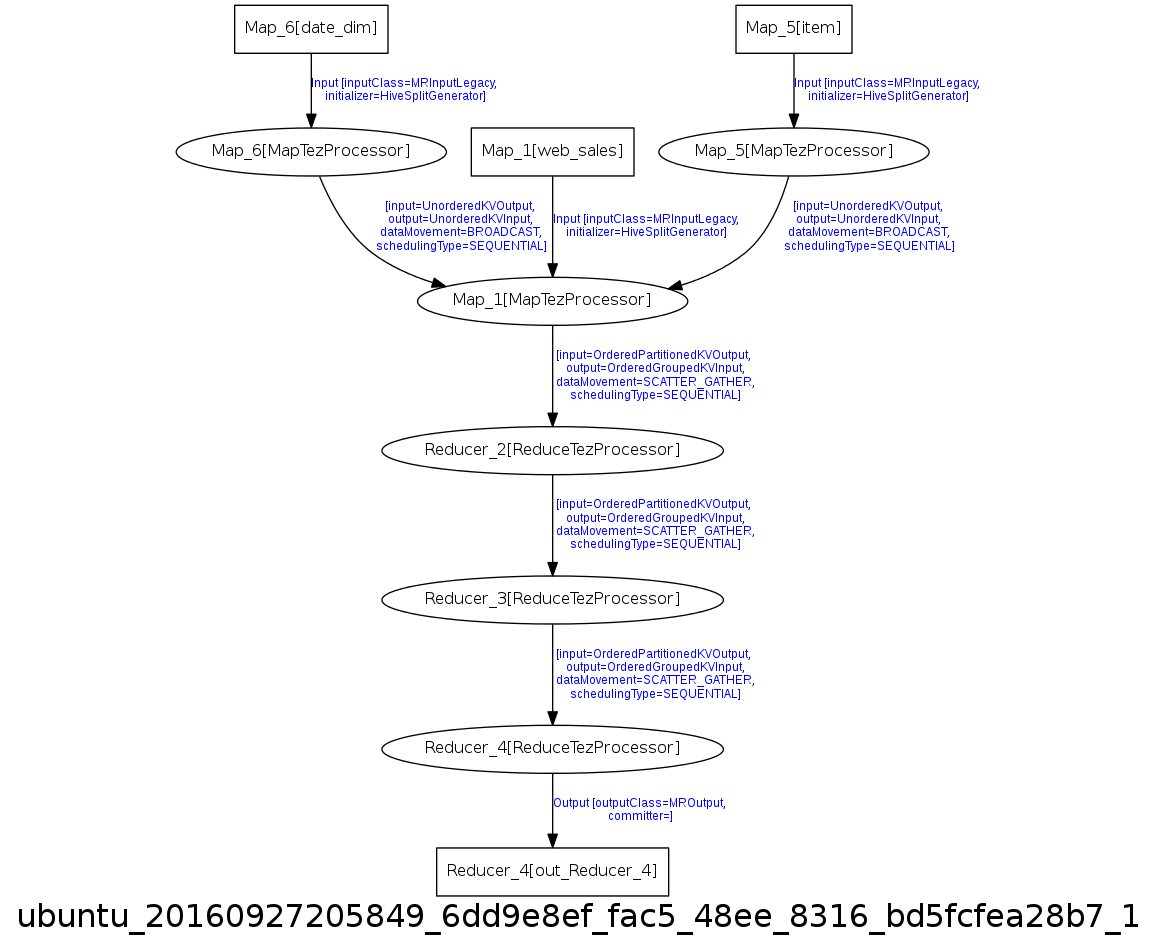
\includegraphics[width=0.85\textwidth]{pic/dag_tez_query12}
\caption{Directed Acyclic Graph (DAG) of Tez (query 12).}
\label{fig:q1d_tez_12}
\end{center}
\end{figure}

\begin{figure}
\begin{center}
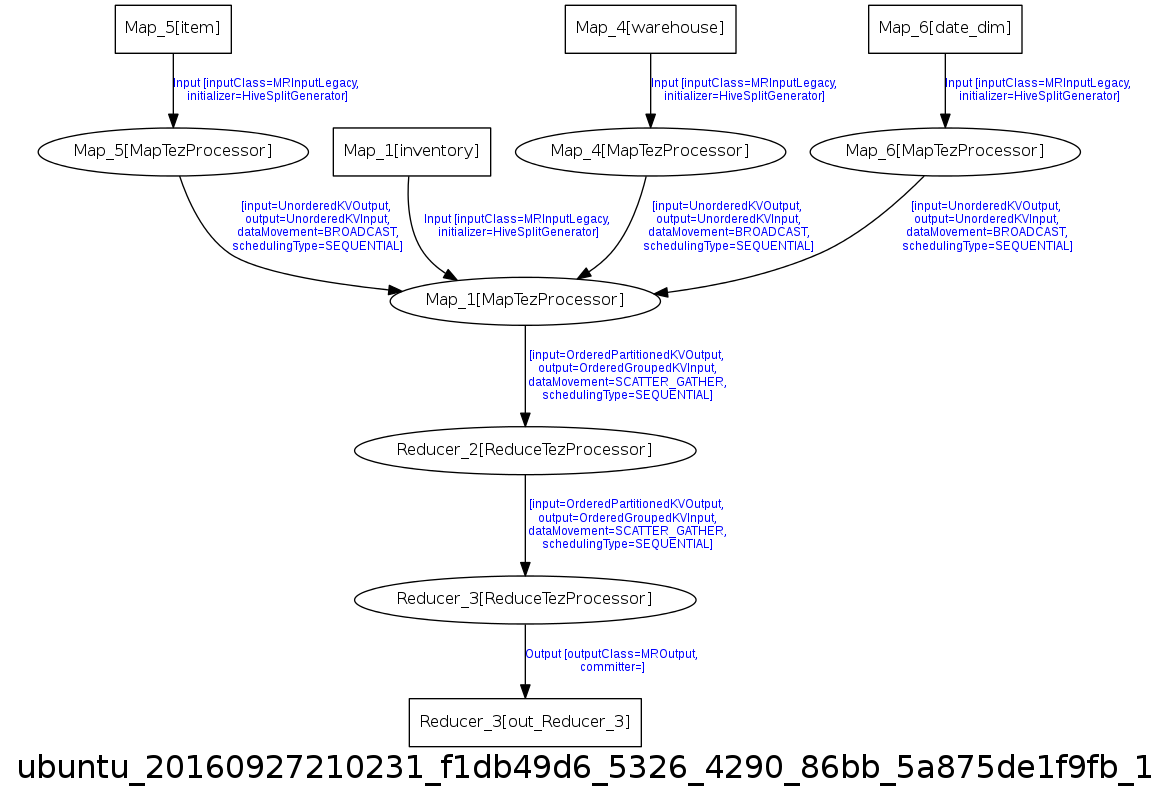
\includegraphics[width=0.85\textwidth]{pic/dag_tez_query21}
\caption{Directed Acyclic Graph (DAG) of Tez (query 21).}
\label{fig:q1d_tez_21}
\end{center}
\end{figure}

\begin{figure}
\begin{center}
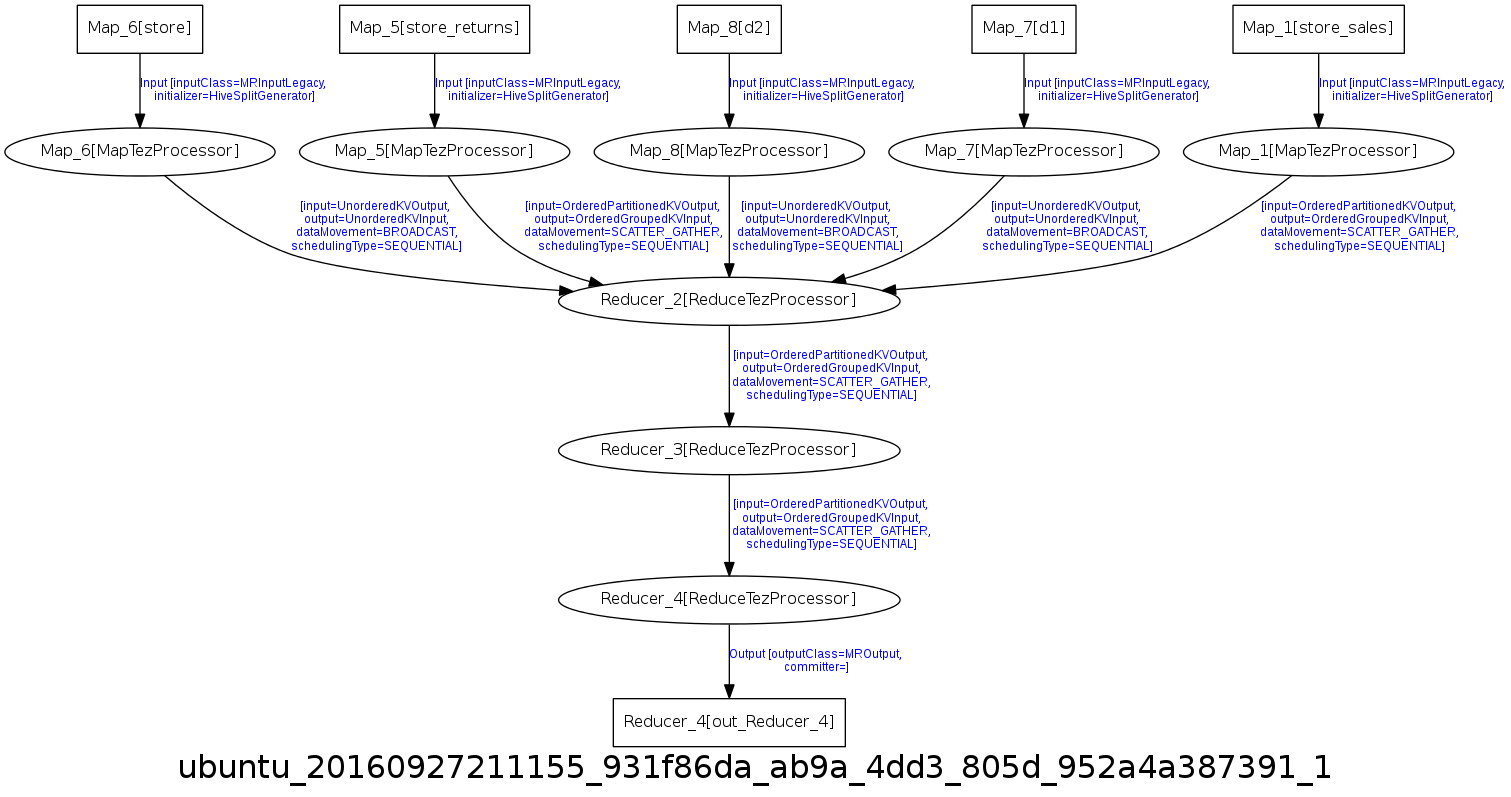
\includegraphics[width=0.85\textwidth]{pic/dag_tez_query50}
\caption{Directed Acyclic Graph (DAG) of Tez (query 50).}
\label{fig:q1d_tez_50}
\end{center}
\end{figure}

\begin{figure}
\begin{center}
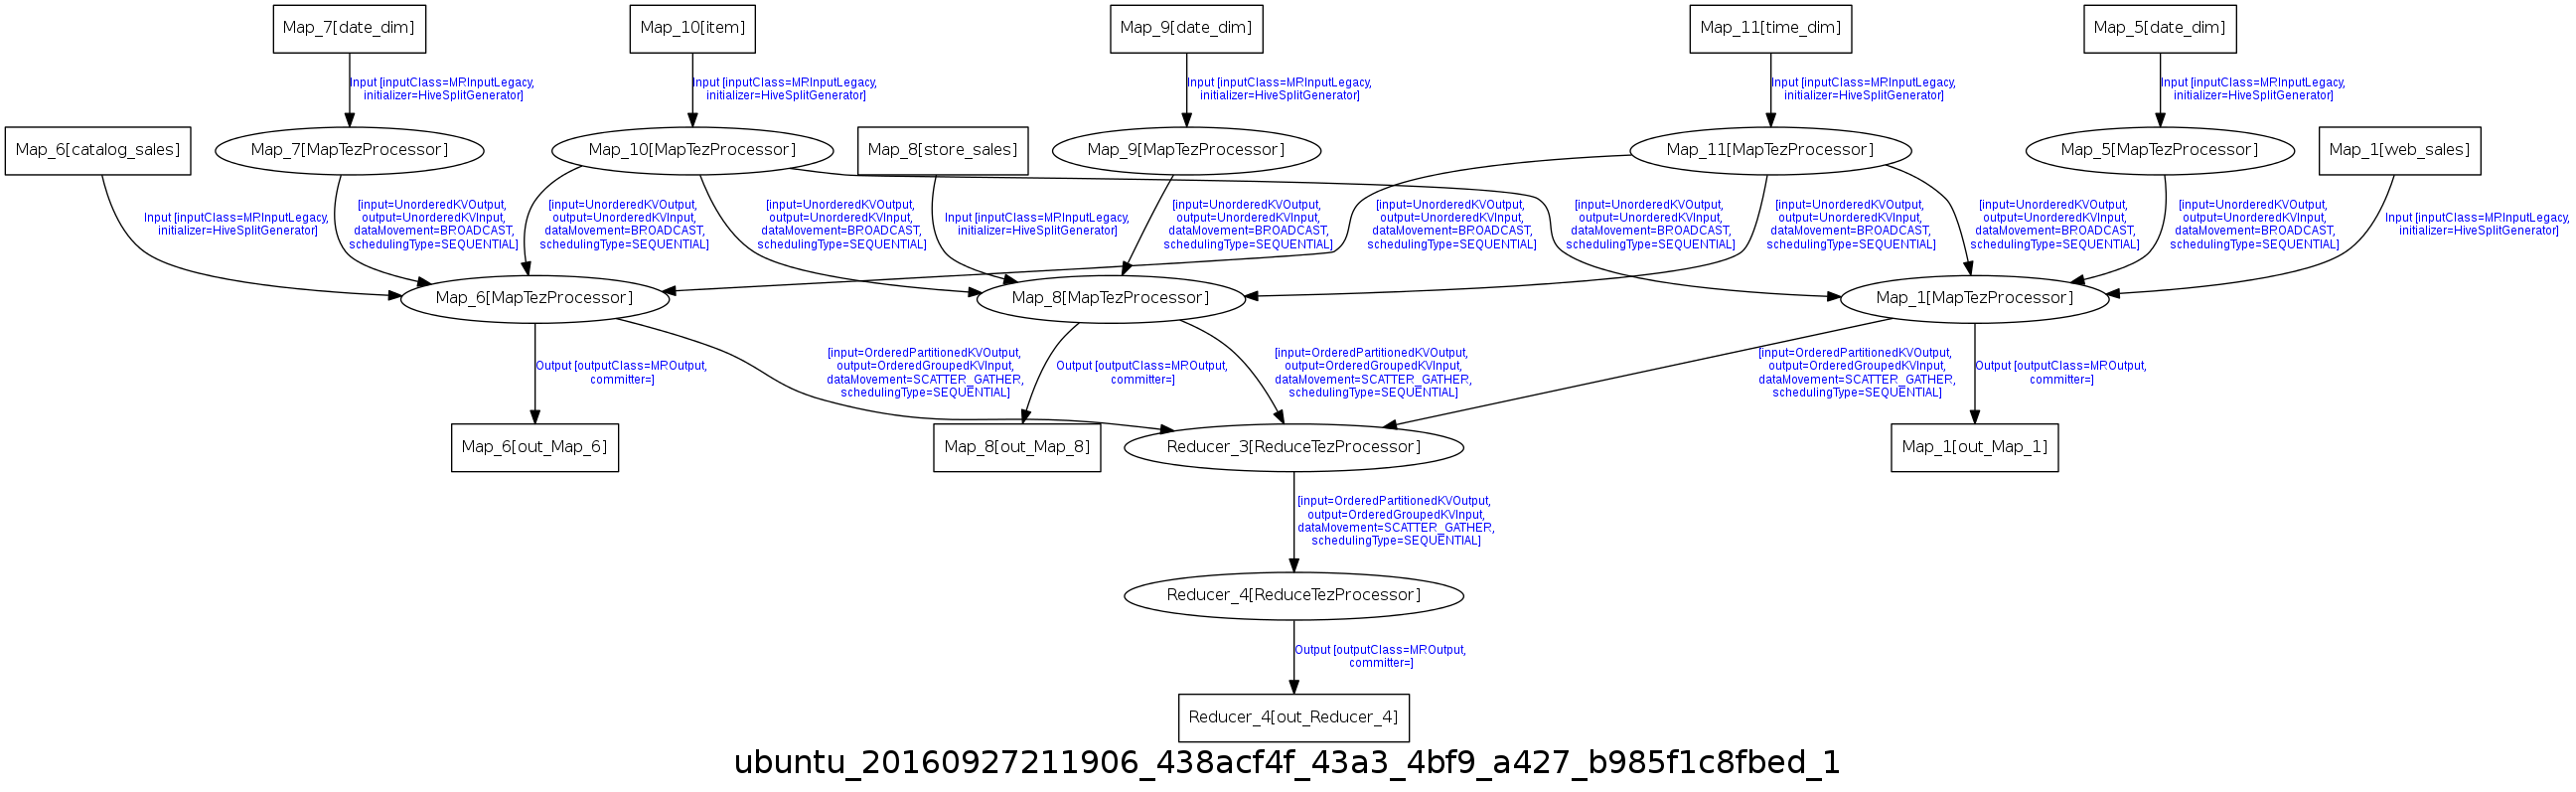
\includegraphics[width=0.85\textwidth]{pic/dag_tez_query71}
\caption{Directed Acyclic Graph (DAG) of Tez (query 71).}
\label{fig:q1d_tez_71}
\end{center}
\end{figure}

\begin{figure}
\begin{center}
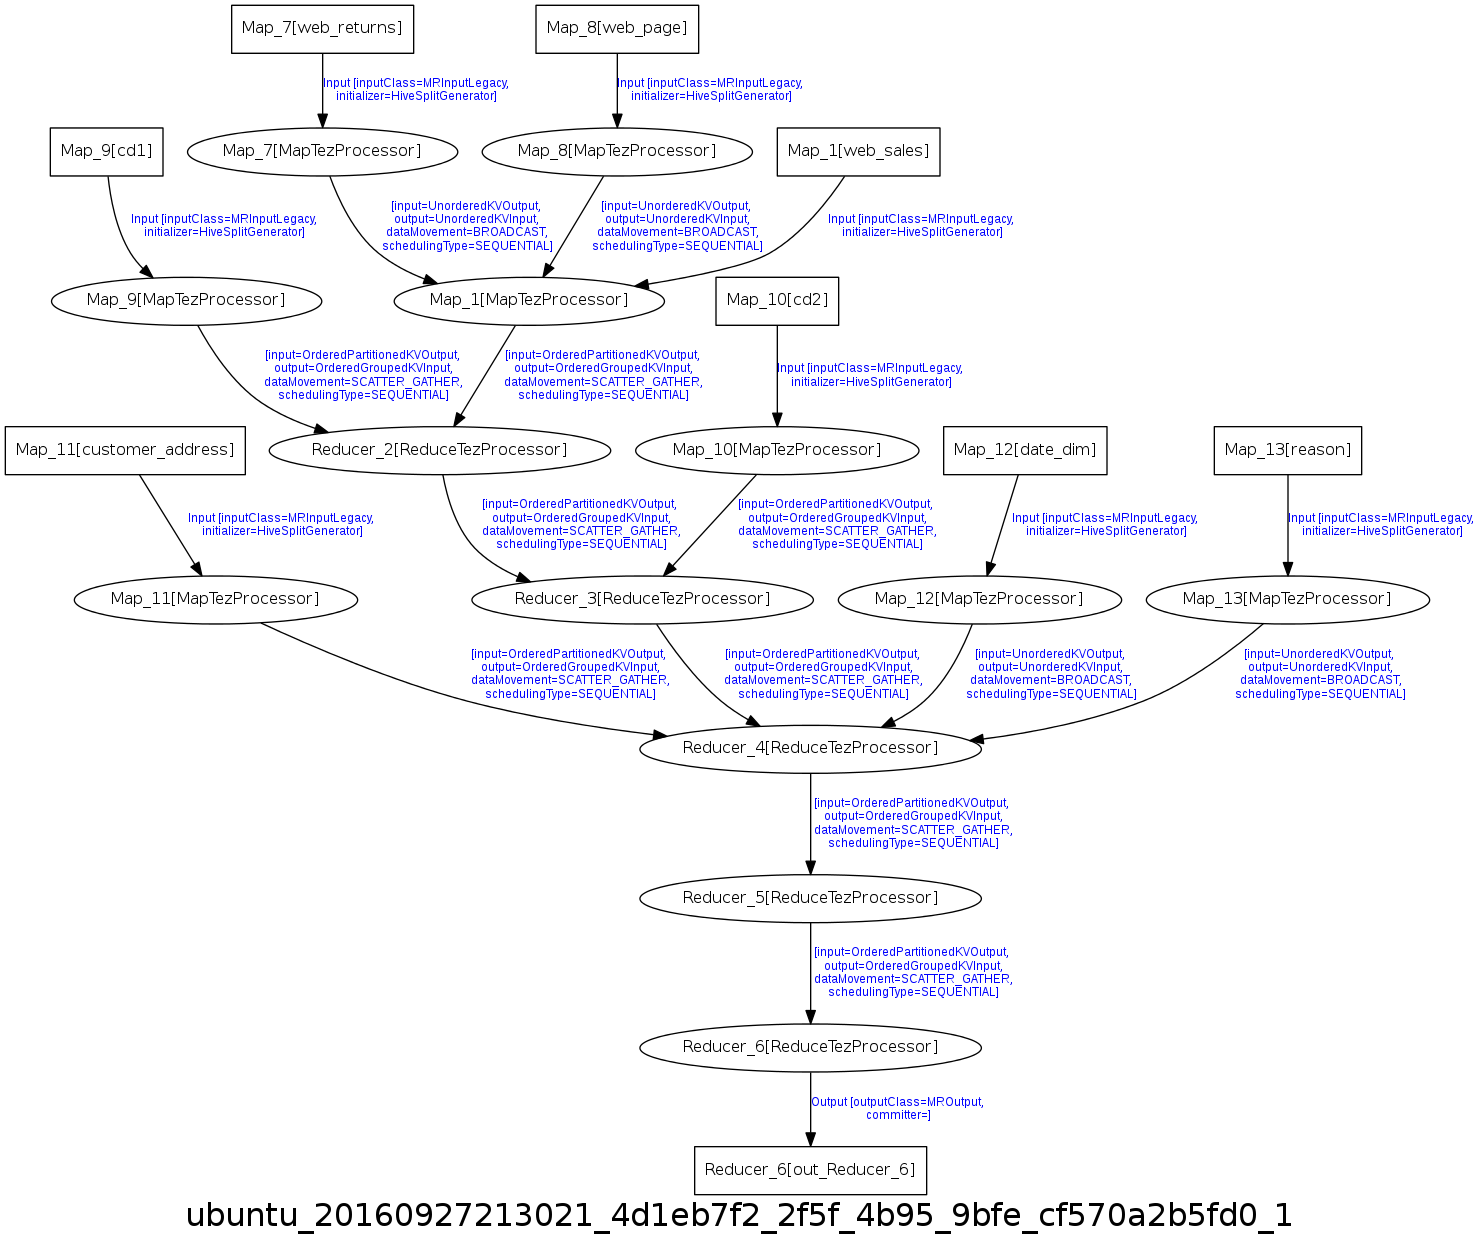
\includegraphics[width=0.85\textwidth]{pic/dag_tez_query85}
\caption{Directed Acyclic Graph (DAG) of Tez (query 85).}
\label{fig:q1d_tez_85}
\end{center}
\end{figure}



%----------------------------------------------------------------------------------------
%	SECTION 3
%----------------------------------------------------------------------------------------

\section{Experiments with Various Parameters}

~~~~~In this section, we picked up query 21 and varied some specific parameters to see whether the performance will improve or not.

\subsection{Hive/MR}
\subsubsection{Number of Reducers}
~~~~~In this experiment, we varied the number of reducers of MR jobs. For each set of parameters, we ran three times and took the average time. The results are shown in the Table\ref{tab:num_of_reducers}

\begin{table}[htbp]
  \centering
  \caption{Number of Reducers and Completion Time}
    \begin{tabular}{rrrrr}
    \toprule
    \# Reducers & 1     & 5     & 10    & 20 \\
    \midrule
    Time (s) & 184.3 & 188.3 & 190.3 & 195.6 \\
    \bottomrule
    \end{tabular}%
  \label{tab:num_of_reducers}%
\end{table}%

As we can see from Table\ref{tab:num_of_reducers}, completion time grows as the number of reducers increases.

\subsubsection{Number of Shuffle Parallel Copies}

~~~~~This time we tuned the number of parallel transfers during the shuffle phase. Also, for each set we ran 3 times and then took the average.

\begin{table}[htbp]
  \centering
  \caption{Number of Shuffle Parallel Copies and Completion Time}
    \begin{tabular}{rrrrr}
    \toprule
    \# Copies & 5     & 10    & 15    & 20 \\
    \midrule
    Time (s) & 184.3 & 183.8 & 186.6 & 188.5 \\
    \bottomrule
    \end{tabular}%
  \label{tab:num_of_parallel}%
\end{table}%

From Table\ref{tab:num_of_parallel}, we can see there is a trend that with the rising of parallel copies, performance tends to decrease.

\subsubsection{Value of Slow Start}
~~~~~Finally, we tried different value on slow start property. The results are shown below.
\begin{table}[htbp]
  \centering
  \caption{Value of Slow Start and Completion Time}
    \begin{tabular}{rrrrrr}
    \toprule
    Value of Slow Start & 0.05  & 0.25  & 0.5   & 0.75  & 1 \\
    \midrule
    Time (s) & 186.4 & 185.7 & 185.5 & 182.5 & 183.8 \\
    \bottomrule
    \end{tabular}%
  \label{tab:val_of_slow}%
\end{table}%

From Table\ref{tab:val_of_slow}, we can tell that when the slow start is 0.75, it has the best performance and it is better than the default value 1.
 

\subsection{Hive/Tez}
\subsubsection{Container Reuse}
\subsubsection{Number of Shuffle Parallel Copies}

~~~~~This time, we tuned the number of shuffle parallel copies on Tez jobs. 3 Times for each set and completion time is on average. Results are shown in Table\ref{tab:num_shuffle_parallel_tez}

\begin{table}[htbp]
  \centering
  \caption{Number of Shuffle Parallel Copies and Completion Time for Tez}
    \begin{tabular}{rrrrr}
    \toprule
    \# Copies & 5     & 10    & 15    & 20 \\
    \midrule
    Time (s) & 50.36 & 50.7  & 51.81 & 50.57 \\
    \bottomrule
    \end{tabular}%
  \label{tab:num_shuffle_parallel_tez}%
\end{table}%

For Tez, we actually cannot tell there is a trend for performance with the variance of number of shuffle parallel copies. The completion time of them are quite similar with each other. 

\subsection{Are the Best Parameters for Query 21 Still Best for Query 12 and 50?}

\subsubsection{Hive/MR}

~~~~~The best parameters for MR job Query 21 is reducers = 1, parallel copies = 10, slow start = 0.75.

After we applied these parameters on Query 12, the average completion time is 178.044 seconds, which is greater than what we got from part 1 experiments with the default settings, 143.804 seconds.

After we applied these parameters on Query 50, the average completion time is 571.969 seconds, which is greater than what we got from part 1 experiments with the default settings, 409.411 seconds.

Thus, we can tell that it is not the best for Query 12 and 50.

\subsubsection{Hive/Tez}

~~~~~The best parameters for Tez job Query 21 is reducers = 1, parallel copies = 5, which is happens to be the default settings.

After we applied these parameters on Query 12, the average completion time is 72.065 seconds, which is greater than what we got from reducers = 1, parallel copies = 10, 58.263 seconds.

After we applied these parameters on Query 50, the average completion time is 320.048 seconds, which has better performance among other parameters we tried. (326.696 seconds for reducers = 1, copies = 10; 326.113 seconds for reducers = 1, copies = 15; 349.039 seconds for reducers = 1, copies = 20).

Thus, we can tell that it is not the best for Query 12, but best for Query 50.


%----------------------------------------------------------------------------------------
%	SECTION 4
%----------------------------------------------------------------------------------------
\section{Experiments with Slave Failure}
\subsection{Completion Time}

~~~~~This time we compare the performance for MR and Tez, with one dataNode fails at the time of 25 \% completion and 75 \% completion. From the Figure\ref{fig:q3a_time}, we can tell that comparing to the completion time of no failure occurs, one dataNode failure leads to the increase of the completion time. And, it is even more expensive if the failure takes place earlier. As in the results, failure at 25 \% makes the completion time much longer than failure at 75 \%.


\begin{figure}
\begin{center}
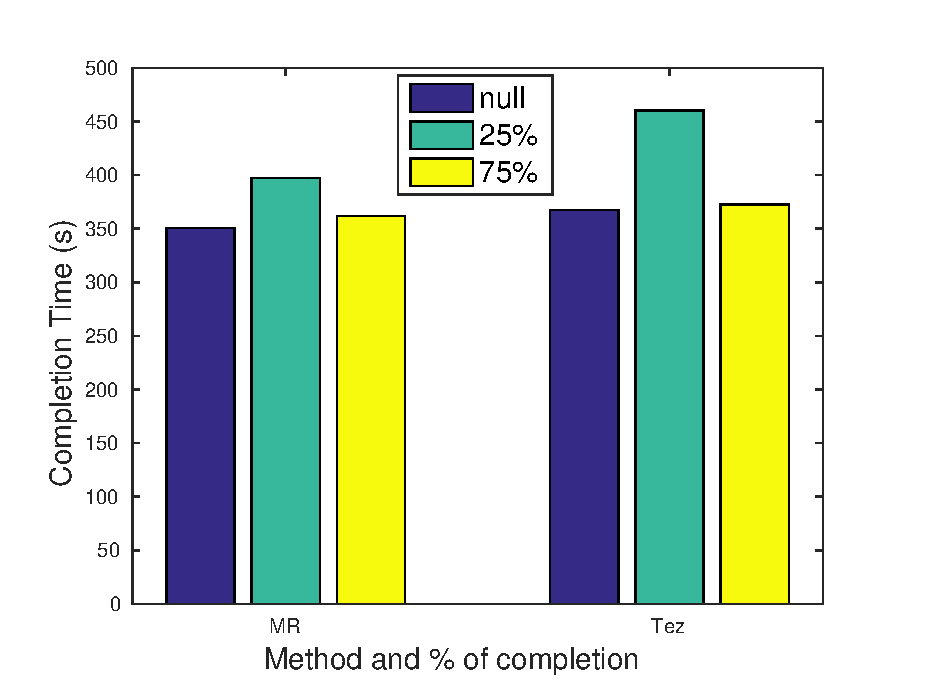
\includegraphics[width=0.85\textwidth]{pic/q3a_time}
\caption{Completion Time of MR and Tez with Failure (query 71).}
\label{fig:q3a_time}
\end{center}
\end{figure}

\subsection{Tasks Variation}

\subsubsection{Hive/MR}
\subsubsection{Hive/Tez}



%----------------------------------------------------------------------------------------
%	SECTION 5
%----------------------------------------------------------------------------------------

\section{Conclusion}



%----------------------------------------------------------------------------------------
%	BIBLIOGRAPHY
%----------------------------------------------------------------------------------------

\bibliographystyle{apalike}

\bibliography{sample}

%----------------------------------------------------------------------------------------


\end{document}